\chapter{Class diagram}
\label{chap:class-diagram}

The purpose of these class diagrams is to give developers an overview of
which classes that is implemented, and the dependencies between the different classes. 

Since the class diagram for the three applications are way to big to display on one A4-page, we felt it 
necessary to split them into several images. 
While the logical view shows dependencies across packages, the class diagrams shows the internal dependencies between
classes. 
Please refer the logical view (Figure \ref{fig:package-diagram-system}) for package dependencies.     


In the next diagrams the following notation is being used:
\begin{itemize}
	\item A solid arrow from class A to class B represents that A uses B.
	\item A dashed arrow from class A to class B represents that A depends on B.
	\item A solid arrow with an arrowhead from class B to class A represents inheritance, that is, B inherits from A.
	\item A dashed arrow with an arrowhead from class B to interface I represents that B implements I.
\end{itemize}

\section{Class Diagram GAPP}
\label{sec:class-diagram-capp}

\paragraph{GAPP - Activities}
Figure \ref{fig:class-diagram-parent-activities} shows the class diagram for the package ``activities''.
This diagram shows the different activities. An activity is, simplified explained, a screen on the application. In section \ref{sec:processView}, the interaction
between different the activities is shown. Since all Activities implements one or more of the interfaces displayed, it
would be completely unreadable to show which activities implement which interfaces. 
The interfaces displayed are standard components in the Android framework, and contains functionality for handling
input. 
The activities get the data that is to be displayed from the packages models, jsonmodels and adapters.    

Figure \ref{fig:activitiy-interaction} shows the different paths to an activity from a user's perspective. 
   
\begin{figure}
	\centering
		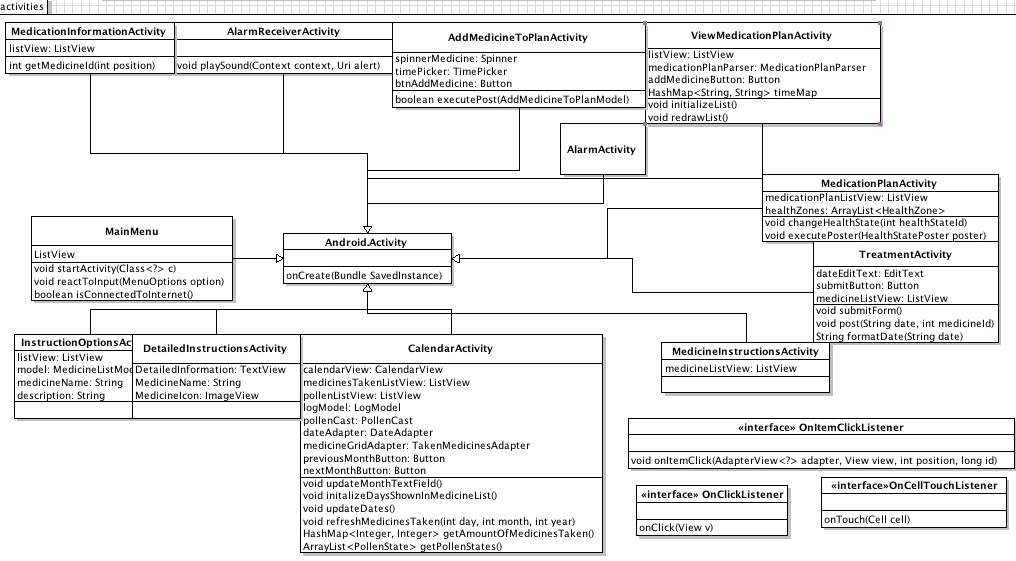
\includegraphics[width = 17.5 cm]{Pictures/ArchPictures/activities.png}
	\caption{Activities in GAPP}
	\label{fig:class-diagram-parent-activities}
\end{figure}

\begin{figure}
	\centering
		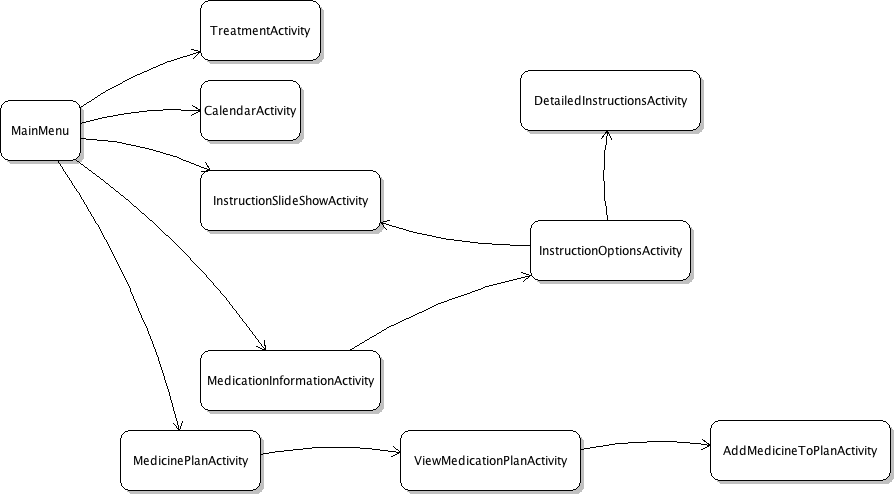
\includegraphics[width = 17.5 cm]{Pictures/ArchPictures/gapparchpictures/ActivityInteractionDiagram.png}
	\caption{Activity interaction GAPP}
	\label{fig:activitiy-interaction}
\end{figure}


\paragraph{GAPP - JSON parsers}
Figure \ref{fig:class-diagram-parent-jsonparsers} shows the class diagram for the package ``jsonparsers''.
This diagram shows the different jsonparser available in the system. In order to make a call to a server in Android, the parsers needs to extend \code{AsyncTask}, which
makes a seperate thread in order to handle the HTTP-calls. The operating system of a device will simply refuse to do network
operations on the main thread.
What we have made, is an abstract generic parser, \code{GenericJSONParser}, which extends \code{AsyncTask} and implements the interface \code{IInitializeFromJSON}.

%TODO: Kanskje flytte det til et sekvensdiagram
When the apllication needs data from the webservice, \code{doInBackground()} is called, which executes the request. 
Once we get a response, \code{initializeDateFromJSON()} is called with the result 
from our http call, in the appropriate class. Each of the subclasses to \code{GenericJSONParser} contains it's own implementation of this method. 

\begin{figure}
	\centering
		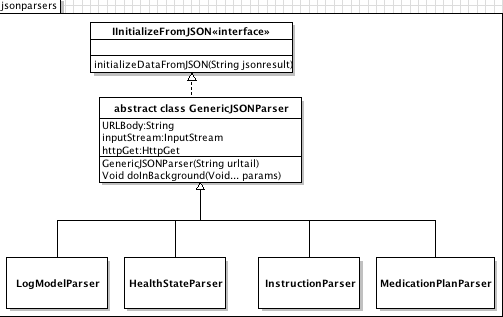
\includegraphics[width = \linewidth]{Pictures/ArchPictures/jsonparsers.png}
	\caption{JSON parsers in GAPP}
	\label{fig:class-diagram-parent-jsonparsers}
\end{figure}


\paragraph{GAPP - JSON posters}
Figure \ref{fig:class-diagram-parent-jsonposters} shows the class diagram for the package ``jsonposters''.
This diagram shows the different posters we have made. These classes are responsible for posting information to the database. As with the parsers, the posters also need to extend \code{AsyncTask}.
The class \code{DatabasePoster} also implements \code{IInitializeFromJSON}. The reason behind this is that once we have made an HTTP-POST, we get a result on JSON-format. The only useful information here is whether
the post was a success or not. There are four subclasses of \code{DatabasePoster}. These classes represent CREATE or DELETE methods towards the database. 

\begin{figure}
	\centering
		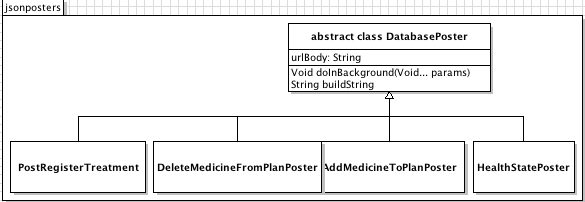
\includegraphics[width = \linewidth]{Pictures/ArchPictures/jsonposters.png}
	\caption{JSON posters in GAPP}
	\label{fig:class-diagram-parent-jsonposters}
\end{figure}



\paragraph{GAPP - jsonmodels}
The data models we are using can be seperated in two categories; ``jsonmodels'' and ``models''. Jsonmodels contains classes
used to hold information retrieved from our webservice.
Models contains classes used to hold information that is independent of which child the application 
displays information about.

 
Figure \ref{fig:class-diagram-parent-jsonmodels} shows the class diagram for the package ``jsonmodels''. 
The different models contains information from database needed in order to display it correctly to the user. This package is used by different activities
in order to display data from the database to users. 
Jsonmodels can be split into two categories; Post models and result models. The postmodels contains an 
important \code{toString()}-method in order to encode the POST parameters correctly. These models are used by the jsonposter-package. 
%TODO: Vanskelig å se hva osm er hva i diagrammet. FIX?
\begin{figure}
	\centering
		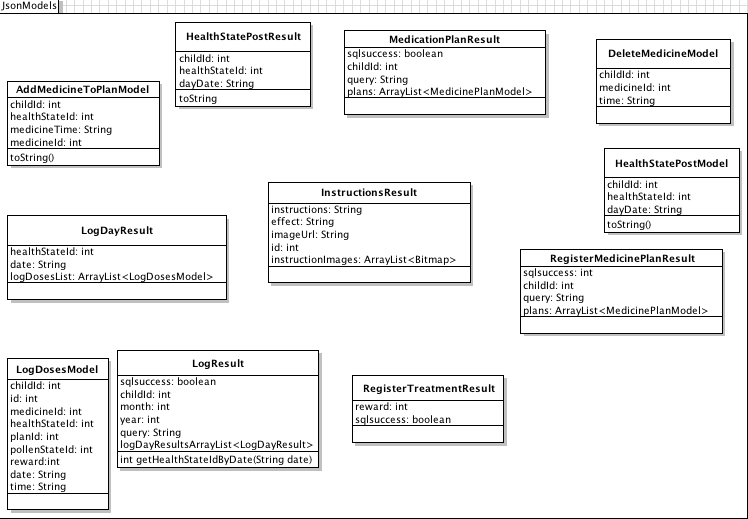
\includegraphics[width = \linewidth]{Pictures/ArchPictures/jsonmodels.png}
	\caption{JSON models in GAPP}
	\label{fig:class-diagram-parent-jsonmodels}
\end{figure}



\paragraph{GAPP - models}
Figure \ref{fig:class-diagram-parent-models} shows the class diagram for the package ``models''
The model package holds three important classes; \code{LogModel}, \code{MedicinePlanModel} and \code{PollenStateAtDayModel}.
\code{LogModel} executes the \code{LogModelParser}, and is used by \code{CalendarActivity}. It contains the amount of each medicine
that is taken on a day, and the health state of the child. \code{MedicinePlanModel} contains the different medicine plans, and \code{PollenStateAtDayModel}
contains information about the pollen distribution at a given day. Note that the latter need some configurations in order to keep up with
``pollenvarslingen.no'', since the application at the time being uses dummy data. The pollen cast from NAAF only contains data about today and tomorrow, so the values collected from this service needs
to be stored in some manner.  
\begin{figure}
	\centering
		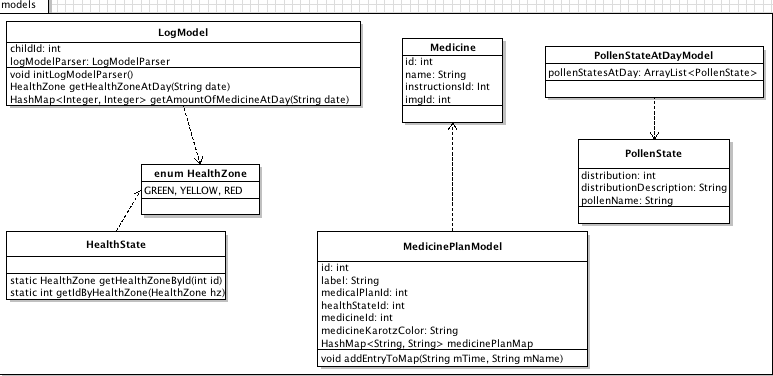
\includegraphics[width = \linewidth]{Pictures/ArchPictures/models.png}
	\caption{Models in GAPP}
	\label{fig:class-diagram-parent-models}
\end{figure}

\paragraph{GAPP - adapters}
Figure \ref{fig:class-diagram-parent-adapters} shows the class diagram for the package ``adapters''.
This package contains some adapters used in order to render ListViews and GridViews correctly.
\begin{figure}
	\centering
		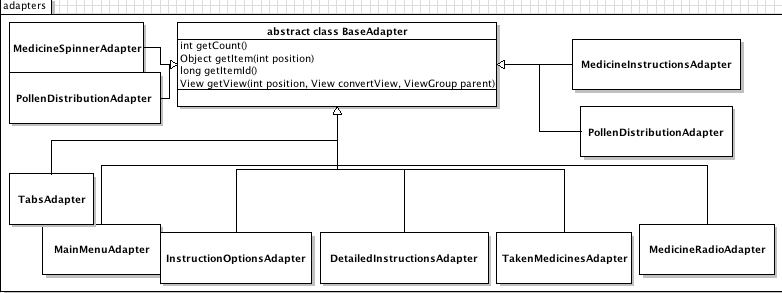
\includegraphics[width = \linewidth]{Pictures/ArchPictures/adapters.png}
	\caption{Adapters in GAPP}
	\label{fig:class-diagram-parent-adapters}
\end{figure}


\paragraph{GAPP - utils, xmlfeed and views}
Figure \ref{fig:class-diagram-parent-extras} shows the class diagram for the packages ``utils'', ``xmlfeed'' and ``views''.
Utils is our ``misc''-package, containing classes we did not know where to put. The \code{DateAdapter} has only one purpose. Convert three integers, 
day, month and year, to an acceptable MySQL-format. The view package contains our only custom view, \code{CalendarView}. This view is opensource and is 
written by Chris Gao (2011)\cite{calendarview}, and is configured by the team to serve our purpose.
\code{CalendarView} and \code{Cell} class is the only views that are programmed. All other views visible to the user is build upon standard Android components like Buttons, ListViews, and so on. 
These files is on XML-format, and are used by the activities to set the content view (the screen image visible to the user). 
These layout-files are not included in the architecture, because it won't actually provide any sorts of useful information to the reader.  

\begin{figure}
	\centering
		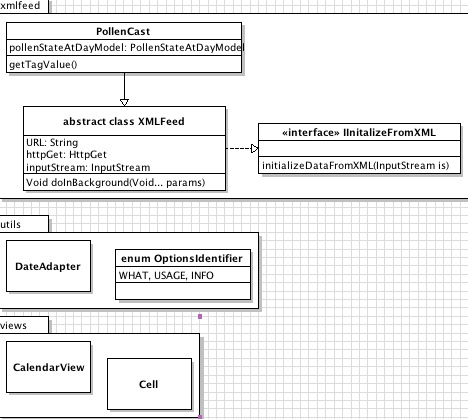
\includegraphics[width = \linewidth]{Pictures/ArchPictures/divclass.png}
	\caption{Other classes in GAPP}
	\label{fig:class-diagram-parent-extras}
\end{figure}

\section{CAPP - Children Application}
The children application also contians to many classes to display in one image, so we have split
this diagram into several images as well.  

\paragraph{CAPP - Activities}
Figure \ref{fig:class-diagram-child-activities} shows the activities in CAPP.
There are four visible activities in CAPP. \code{AlarmReceiverActivity} is an activity that updates the stored alarms in the system. \code{MainMenuActivity}
displays the main menu. \code{InstructionsActivity} contains a slideshow of informative images on how to take medicines correctly. 
\code{DisplayRewardsActivity} shows the collected
stars to the children. \code{DistractionActivity} controls the views when a child is taking a medicine.
\begin{figure}[h!]
	\centering
		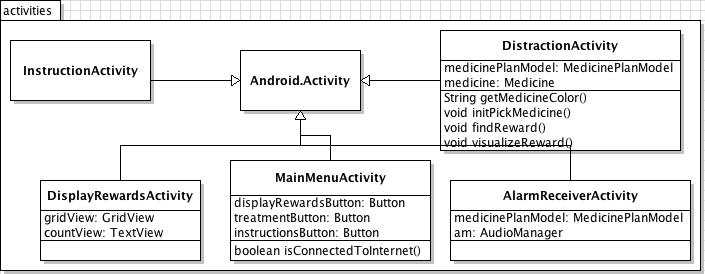
\includegraphics[width = \linewidth]{Pictures/ArchPictures/capparchpictures/capp_activities.png}
	\caption{Activities in CAPP}
	\label{fig:class-diagram-child-activities}
\end{figure}


\paragraph{CAPP - Adapters}
Figure \ref{fig:class-diagram-child-adapters} shows the adapters in CAPP.
CAPP has two adapters. \code{Medicine\-ListAdapter} renders a list of which medications a child can take. 
\code{TabsAdapter} is an adapter fitted for \code{Instructions\-Activity}, and contains the logic behind the slideshow that is displayed.
% \begin{figure}
% 	\centering
% 		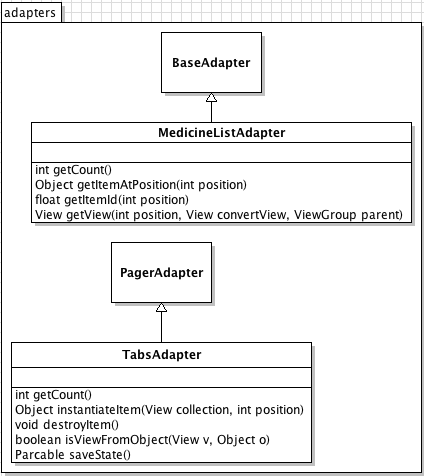
\includegraphics[width = 8.0 cm]{Pictures/ArchPictures/capparchpictures/capp_adapters.png}
% 	\caption{Adapters in CAPP}
% 	\label{fig:class-diagram-child-adapters}
% \end{figure}

\paragraph{CAPP - Models}
Figure \ref{fig:capp-class-models} shows the models in CAPP.
It contains three models. Due to time restrictions, we were not able to extend the application to cover several children.
A model for children must thus be made in future development. 

\begin{figure}
	\begin{minipage}[b]{0.44\linewidth}
		\centering
			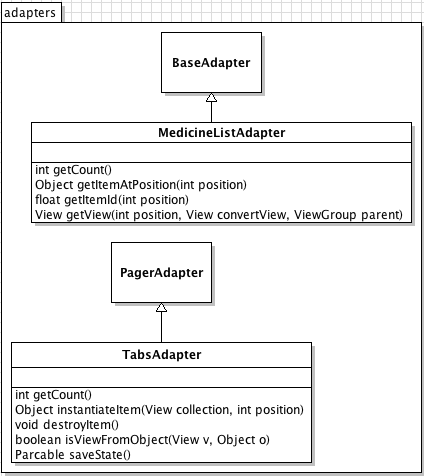
\includegraphics[width=\linewidth]{Pictures/ArchPictures/capparchpictures/capp_adapters.png}
		\caption{Adapters in CAPP}
		\label{fig:class-diagram-child-adapters}
	\end{minipage}
	\hspace{0.1\linewidth}
	\begin{minipage}[b]{0.44\linewidth}
		\centering
		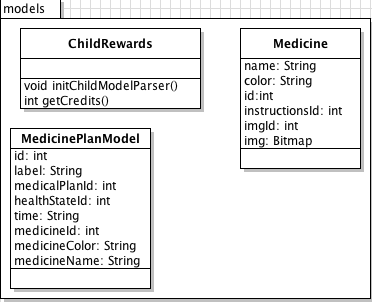
\includegraphics[width=\linewidth]{Pictures/ArchPictures/capparchpictures/capp_models.png}
	\caption{Available plans in GAPP}
	\label{fig:capp-class-models}
	\end{minipage}
\end{figure}

% \begin{figure}
% 	\centering
% 		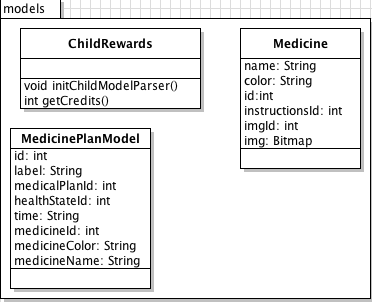
\includegraphics[width = 8.0 cm]{Pictures/ArchPictures/capparchpictures/capp_models.png}
% 	\caption{Models in CAPP}
% 	\label{fig:class-diagram-child-models}
% \end{figure}

\paragraph{CAPP - JsonModels}
Figure \ref{fig:class-diagram-child-jsonmodels} shows the JsonModels in CAPP.
\code{RegisterMedicinePostModel} is used as model for \code{PostRegisterTreatment} that is shown 
in figure \ref{fig:class-diagram-child-jsonposters}
The rest of the models reflects the information stored in the database.
\begin{figure}
	\centering
		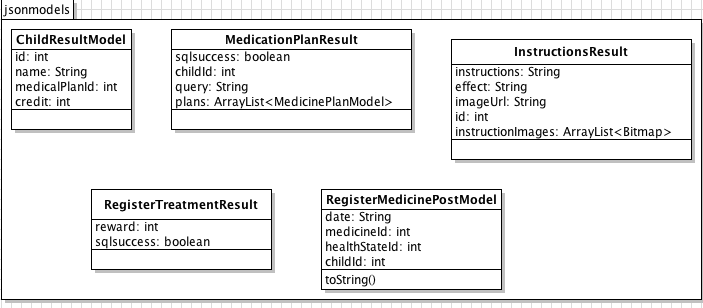
\includegraphics[width = \linewidth]{Pictures/ArchPictures/capparchpictures/capp_jsonmodels.png}
	\caption{JsonModels in CAPP}
	\label{fig:class-diagram-child-jsonmodels}
\end{figure}

\paragraph{CAPP - JsonParsers}
Figure \ref{fig:class-diagram-child-jsonparsers} shows the JsonParsers in CAPP.
It is worth mentioning that \code{DownloadImageTask} and \code{InstructionsParser} is not currently used. 
At the start of the project, the customer wanted easily modifiable instructions for the children. We thought it 
might be useful to implement classes that could download instructions from the web. However, the customer never 
created these online instructions. We thought it might be useful for future developers to extend these classes
if such functionality is needed one day.   


\begin{figure}
	\centering
		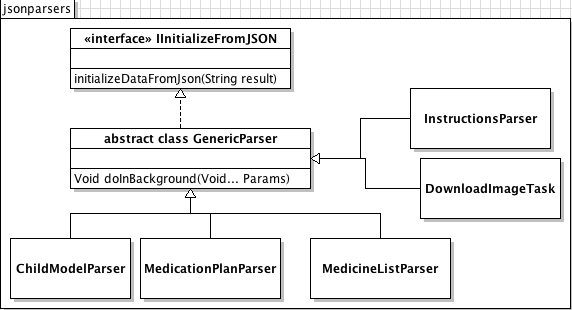
\includegraphics[width = \linewidth]{Pictures/ArchPictures/capparchpictures/capp_jsonparsers.png}
	\caption{JsonParsers in CAPP}
	\label{fig:class-diagram-child-jsonparsers}
\end{figure}

\paragraph{CAPP - JsonPosters}
Figure \ref{fig:class-diagram-child-jsonposters} shows the JsonPosters in CAPP.
The application does a HTTP POST is when a mediciation is completed. For consitency among CAPP and GAPP,
this package contains similar classes as those found in GAPP. 

\begin{figure}
	\begin{minipage}[b]{0.44\linewidth}
		\centering
			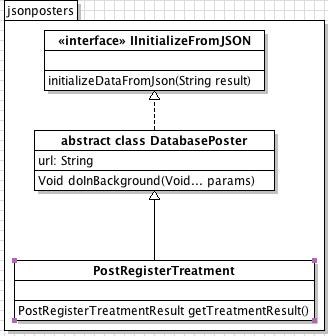
\includegraphics[width=\linewidth]{Pictures/ArchPictures/capparchpictures/capp_jsonposters.png}
		\caption{JsonPosters in CAPP}
		\label{fig:class-diagram-child-jsonposters}
	\end{minipage}
	\hspace{0.1\linewidth}
	\begin{minipage}[b]{0.44\linewidth}
		\centering
			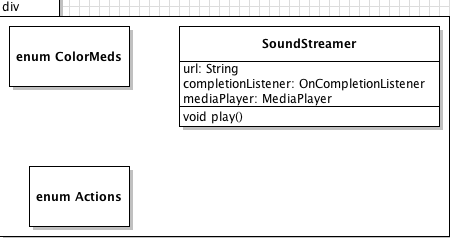
\includegraphics[width=\linewidth]{Pictures/ArchPictures/capparchpictures/capp_div.png}
		\caption{Misc classes in CAPP}
		\label{fig:class-diagram-child-misc}
	\end{minipage}
\end{figure}

% \begin{figure}
% 	\centering
% 		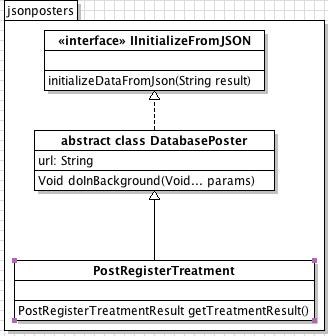
\includegraphics[width = 8.0 cm]{Pictures/ArchPictures/capparchpictures/capp_jsonposters.png}
% 	\caption{JsonPosters in CAPP}
% 	\label{fig:class-diagram-child-jsonposters}
% \end{figure}
% 
%  
% \begin{figure}
% 	\centering
% 		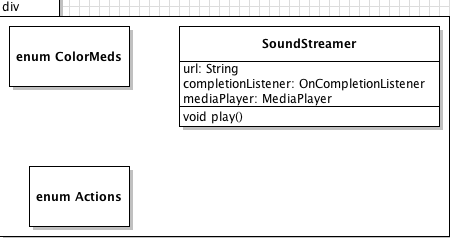
\includegraphics[width = 8.0 cm]{Pictures/ArchPictures/capparchpictures/capp_div.png}
% 	\caption{Misc classes in CAPP}
% 	\label{fig:class-diagram-child-misc}
% \end{figure}


\paragraph{CAPP - Services}
Figure \ref{fig:class-diagram-child-services} shows the services in CAPP.
As defined by Android\cite{androidservice}, a \code{Service} is an application component representing either an application's desire to perform a longer-running operation while not interacting with the 
user or to supply functionality for other applications to use.
We have implemented two services, \code{OnBootReceiver} and \code{AlarmUpdateReceiver}. \code{OnBootReceiver} is used to gather alarm information from the database once a device is turned on.
AlarmUpdateReceiver has similar functionality. It deletes old alarms, and sets the new alarms.
\clearpage{}
\begin{figure}
	\centering
		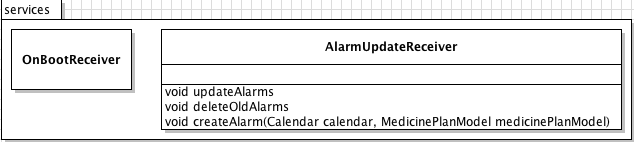
\includegraphics[width = \linewidth]{Pictures/ArchPictures/capparchpictures/capp_services.png}
	\caption{Services in CAPP}
	\label{fig:class-diagram-child-services}
\end{figure}

\section{Karotz Application}

Figure \ref{fig:class-diagram-karotz} shows the class diagram for the Karotz app. There are strong relations between all the modules in the ``src''
package. The \code{Blopp} class is instantiated when the application is started and has the responsibility of invoking all the necessary modules. It maintains a \code{Repository}
for connecting to the database. The repository depends on the \code{Notification} module for calling the method \code{makeNotification()} which creates a timeout of a given
length. The repository ensures that the method is only called for the nearest scheduled medication, and overwrites all the previously set notification timeouts. When
a notification event is initiated, the application calls \code{startMedication()} in the \code{Medication} module. The distraction process uses the functions \code{doseListToManuscript()} 
and \code{interpretAction()} in the module \code{util} for creating a list of actions required by the manuscript, and performing them. Action descriptions are stored in an external configuraton
file, which is loaded in the \code{Blopp} module in the field \code{config}. When a medication is finished, \code{endMedication()} calls \code{logMedicineTaken()} in \code{Repository}
once for each medicine that was taken.

\begin{figure}
	\centering
		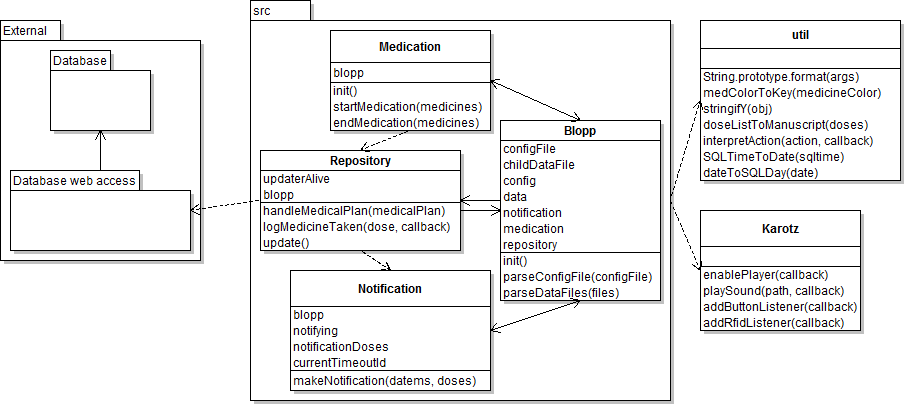
\includegraphics[width = \linewidth]{Pictures/ArchPictures/KarotzClassDiagram.png}
	\caption{Class diagram for the Karotz application}
	\label{fig:class-diagram-karotz}
\end{figure}
%INSERT DESCRIPTION WHEN MORE IS KNOWN ABOUT IT!!